Generating the optimal constant value in an expression tree is a hard problem for GP. In contrast to the discrete problem of selecting and combining from a limited set of base functions, the selection range of a constant value is huge. In this section we cover our approach to this problem.
A constant value can appear in an expression tree as a linear weight for a base function, or as a leaf. The following clarifies the difference. In $ f(x) = \sin(\log(2, x))$ the value of 2 is a constant value, while in $ g(x) = 3.14 sin(x) + 4.25 cos(x)$ the 3.14 and 4.25 are linear weights. In our implementation, the tree encoding has a hidden linear weight for each node which can be optimized independently from constant arguments. When we refer to constant optimization, we are referring to the process of finding the optimal values of constant values in the expression.
The size of the constant set dominates the size of the search space. We intentionally restrict this set to [0,1]. This reduces the size of c from $2^{64}$ to $2^{23}$ since we use the IEEE 754 double representation. This restriction in range does not prevent larger constants from being evolved. The algorithm will evolve subtrees combining base functions with constants in order to find more optimal values.
An expression tree is constant if all its children are constant expression trees. As a base case, a leaf node is a constant expression if it is not a feature. This problem statement allows us to define a recursive algorithm to detect constant expressions. It should be noted that its complexity is O(n) only in the worst case, in the degenerate case where the entire tree is a constant expression. Upon detecting a non constant subtree, the algorithm returns early without a full traversal. 
Using the checking procedure a tree marked as a constant expression is not allowed in the initialization procedure. It is still possible to create constant expressions by applying crossover. The mutation operator will not generate constant subtrees. Our tool does not prevent constant expressions from forming in this way, the evaluation step following crossover will filter out the constant expressions using evolutionary pressure. A tree can contain subtrees that represent constant expressions. This is an immediate effect of the GP algorithm trying to evolve the optimal constant. This can lead to large subtrees that can be represented by a single node. Nodes used in such a constant subtree are not available for base functions and therefore present a waste in memory and evaluation cost. There is a counterargument to be made here: parts of a constant subtree can help evolve constants faster than random selection. It is therefore possible that folding such subtrees can lead to worse fitness values. We can use a depth sensitive objective function to try to mitigate this effect, but a more direct approach is replacing the subtrees. Using the previous constant expression detection technique we can collect all constant subtrees from a tree and replace it with the constant value they represent, which we will refer to as folding.
\begin{figure}
	\centering
    \begin{subfigure}{0.5\textwidth}
    \centering
    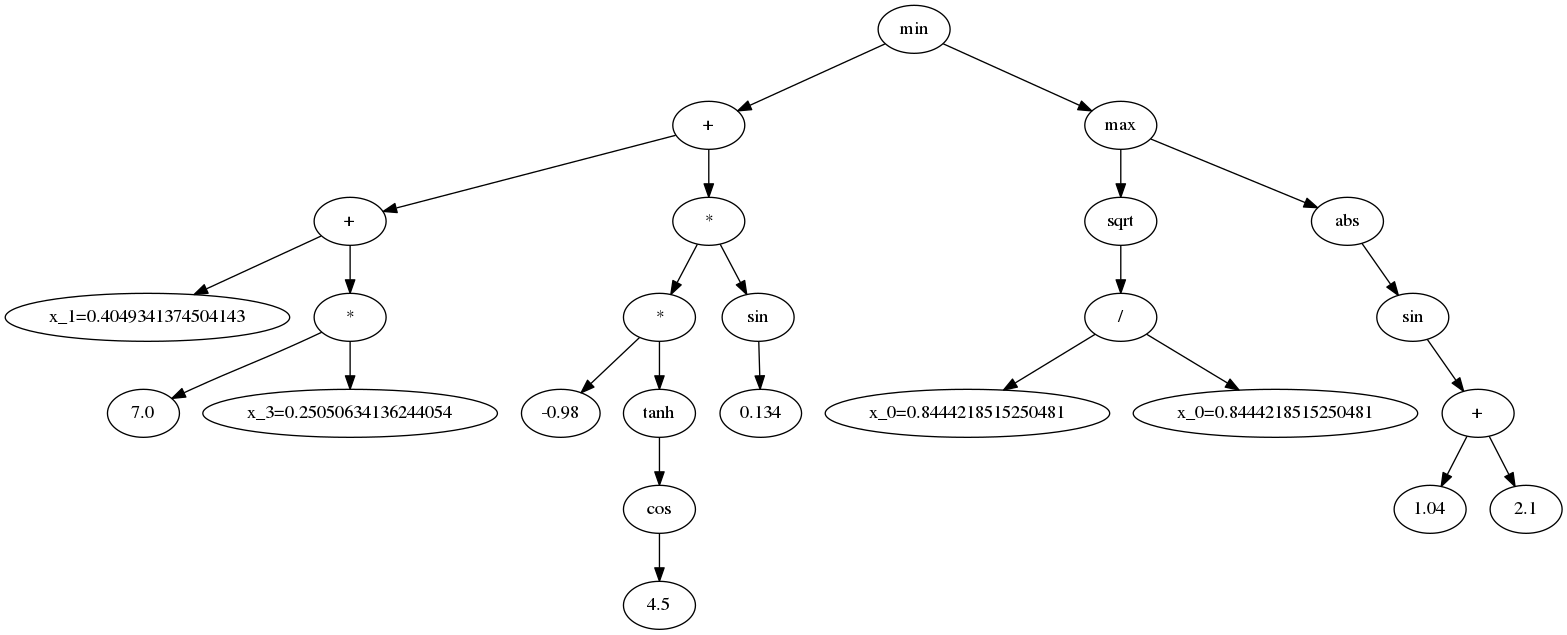
\includegraphics[width=\textwidth,height=\textheight,keepaspectratio]{figures/prefold.png}
    \caption{Tree before subtree folding.}
	\end{subfigure}
	\begin{subfigure}{0.5\textwidth}
    \centering
    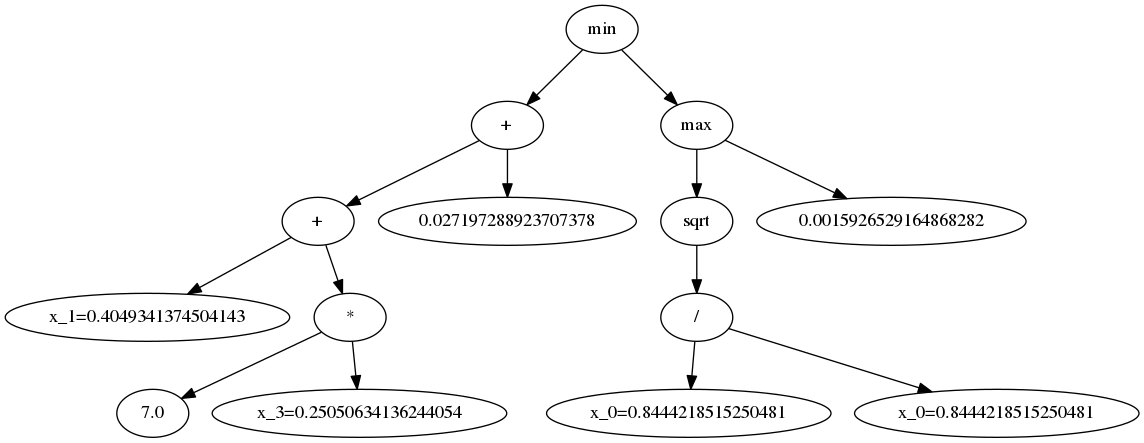
\includegraphics[width=\textwidth,height=\textheight,keepaspectratio]{figures/postfold.png}
    \caption{Tree after subtree folding.}
	\end{subfigure}
	    \caption{Constant subtree folding.}
    \label{fig:folding}
\end{figure}
We found that constant folding can have a negative effect on convergence in some cases. A constant subtree with depth d represents between d and $2^{d+1}-1$ constants. Both mutation and crossover can use these constants to generate more expressive trees. Constant folding is a trade-off between this expressive power and time and space complexity. More importantly, constant folding is a necessity in order to optimize the constant values with a continuous optimizer. It reduces the dimensions of the optimization problem significantly. In Figure \ref{fig:folding} we see the effect of applying the constant subtree folding. 
\subsection{Optimizers}
Using a continuous optimizer in combination with GP is a known solution \cite{GEDE, GPConst} to the constant optimization problem.
Selecting which algorithm to combine with GP is a difficult question and, to our knowledge, no comparative study is available. Given a tree with k constant leaves and all constant subtrees folded, we would like to find the optimal values for those constants. In most optimization problems an initial solution is not provided, only the problem domain and an objective function. However, we do have an initial solution, namely that generated by GP. Instead of choosing random points in the search space, we therefore opt to perturb this initial solution. In order to make a fair comparison between the algorithms, they are, to the extent possible configured similarly. Based on the optimal value for PSO \cite{PSO} we use a default population of 50. The iterations are set at 50. We can apply the optimizer on each expression each iteration or only on a selection of the best expressions at each iteration or only at the end of a phase on all, a selection, or only the best expressions. In our experiments we will show the effect on convergence of these choices.
\subsubsection{ABC}
Artificial Bee Colony \citep{ABC} is a relatively new nature inspired algorithm. It is not limited to continuous optimization, and has even been used for symbolic regression itself \cite{ABCSR}. A key advantages over other algorithms is a low parameter count. ABC is good at exploration (thanks to its scouting phase) though sometimes lacking in exploitation. To resolve this, ABC can be combined with more exploitative algorithms \citep{ABCPSO}.
ABC uses three distinct phases per iteration. It maintains a set of potential solutions and a population of particles. Each particle is either employed, onlooker, or scout. An employed particle perturbs a known solution and replaces it if an improvement in fitness is obtained. If this fails for a preset number of iterations, the solution is marked exhausted and a new one scouted. Scouting in this context is generating a new potential solution. After the employed phase, the onlooking particles decide, based on a fitness weighted probability, which solutions should be further optimized. In contrast to the employed particles the onlooking particles swap out solutions each iteration. Finally, exhausted solutions are replaced by scouted solutions.
The algorithm initializes its solution set by multiplying each constant with a random number $\in [-1,1]$. Each instance records its best solution. We use the initial value of each constant as the mean of a normal distribution and generate values within 2 standard deviations. A configurable scaling factor is introduced, in our test problems we use 20. This value is a trade-off between exploration and an increasing probability for generating invalid solutions. A solution is updated if its fitness improves. The new fitness weights for the roulette wheel selection are calculated and the global best is updated. Unlike PSO, a solution is only updated if an improvement is measured. In contrast to DE, equal fitness values do not lead to an update. An equality update allows an optimization algorithm to cross zero gradient areas in the fitness landscape. The influence solutions have on each other in ABC is not as great as in DE. In PSO, the entire position, in all dimensions, is updated. In DE this depends on a parameter. This distinction can have a large impact on convergence and is determined by the correlation or separability of each constant.
We do not know in advance if our problem instances are separable or not. The configuration of our tool for ABC is: 
\begin{itemize}
\item limit = 0.75 * onlookers / 2 : If a solution does not improve after this many iterations, it is marked exhausted. This limit is scaled by the number of dimensions per instance. 
\item population = 50 solutions.
\item onlookers = 25 : The number of onlookers. Setting this value to half that of the employed finds a balance between exploitation and evaluation cost.
\item employed = 50 
\item scouts = 25 : This is a maximum number of scouts used after a solution is exhausted. 
\end{itemize}
This configuration is guided by the findings in \cite{ABC}. Compared to PSO and DE,a single iteration in ABC will have more optimization per solution, but on fewer dimensions.
\subsubsection{PSO}
Particle Swarm Optimization \cite{PSO} is one of the oldest population based metaheuristics. It consists of particles that share information with each other about the global best solution.
Each particle is assigned a position in the n-dimensional search space. A particle's position is updated using its velocity which is influenced by information from the global best and the local best. The concept of inertia is used to prevent velocity explosion \cite{PSOExplosion}.
Each particle is given a random location at start. Similar to our ABC imlementation, we perturb the known solution with a random value $\in [0,1]$.
To avoid premature convergence each particle is assigned a small but non-zero velocity. Without this velocity all particles are immediately attracted to the first global best. 
The algorithm updates all particles in sequence by updating each velocity using a weighted sum of local and global best, then updating its position using the velocity.
The configuration of our tool for PSO is:
\begin{itemize}
\item $C_1, C_2$ = 2, weights for global and local best position differences, recommended in \cite{PSOParameter}.
\item $w_i = \frac{1 + r}{2}$ with r random $\in [0,1]$ : A random inertia weight leads to faster convergence for a generic problem set \cite{PSOInertia}.
\item $R_1, R_2$ r with r random in [0,1], random weights for the global and local best positions. 
\item population = 50 : PSO is not sensitive to populations larger than this value \cite{SwarmIntelligence}.
\end{itemize}
CSRM's optimizer does not impose constraints on the domain of each constant. Finding the domain of a constant in the expression tree requires a domain analysis of the expression tree. Finding the exact domain is infeasible, given that some of the data points for features are unknown (e.g. validation or test data). It is thus possible that a particle obtains values outside the valid domain of one or more constants, resulting in an invalid expression tree. If so, the particle temporarily no longer contributes to the search process.
\subsubsection{DE}
Differential Evolution is a vector based optimization algorithm, operating by computing the difference between particles. The algorithm has a population of n vectors and holds a linear set of values to optimize, one per dimension. Similar to our approach in initializating PSO and ABC, we perturb a known (sub)optimal solution. A vector stores its current value, and the best value. CSRM uses a DE/rand/2/bin configuration. The notation indicates a random selection of (2) vectors with binomial crossover. This configuration is referenced \cite{DE} as one of the most competitive for multimodal problems with good convergence characteristics to the global optimum. Each iteration the algorithm processes all vectors. First a mutation step obtains a new vector based on the difference of 2 randomly selected, with replacement. Then we apply a binomial crossover operation. Finally we compare with the new vector and replace it if it has the same or better fitness, in contrast to PSO and ABC. The equality update allows DE to traverse zero gradient areas in the search space.
The configuration of our tool for DE is:
\begin{itemize}
\item F = 0.6 : Weight determines the mutation step. The value of 0.6 is reported as a good starting value\citep{DESurveyLatest}. 
\item Cr = 0.1 : The Cr value influences the crossover step. It should be in [0,0.2] for separable functions, and [0.9, 1] for non-separable functions. We cannot assume dependency between the constants, and therefore use 0.1. This results in DE focussing along the axes of each dimension in its search trajectory. 
\end{itemize}
Compared to PSO DE has a low parameter count, optimal values for these parameters can be found in literature \cite{DESurveyLatest}. The population size should be t * d with t in [2, 10]. Since we do not know d in advance, and to keep the comparison fair we set the population at 50, allowing for optimal values for up to 25 dimensions (constants).